\chapter{INCL 4.2 Cascade and ABLA V3 Evaporation with Fission}

\section{Introduction}

There is a renewed interest in the study of spallation reactions. This
is largely due to new technological applications, such as Accelerator
Driven Systems, consisting of sub-critical nuclear reactor and
particle accelerator. These applications require optimized spallation
targets or spallation sources. This type of problem has typically a large number
of parameters and thus it cannot be solved by trial and error
method. One has to rely on simulations, which implies that very
accurate simulation tools need to be developed and their validity and
accuracy needs also to be assessed.

Above the energy 200 MeV it is necessary to use reliable models due to
the prohibitive number of open channels. The most appropriate modeling
technique in this energy region is intra-nuclear cascade (INC) combined
with evaporation model. One such pair of models is the Li\`ege cascade
model INCL4.2 coupled with ABLA evaporation model. The strategy adopted
by the INCL4.2 cascade is to improve the quasi-classical treatment of
physics without relying on too many free parameters. 

This chapter introduces the physics provided by INCL4.2 and ABLA V3 codes as implemented in Geant4.
Tables \ref{tbl:inclsummary} and \ref{tbl:ablasummary} will summarize the key features 
and provides references describing in detail the physics.


\section{INCL4.2 cascade} 
\label{sec:inclmodel}

INCL4.2 is a Monte Carlo simulation incorporating aforementioned cascade
physics principles. INCL4.2 cascade algorithm consists of an
initialization stage and the actual data processing stage.


The INCL4.2 cascade can be used to simulate the collisions between
bullet particles and nuclei. The supported bullet particles and the
interface classes supporting them are presented in table
\ref{tbl:inclsummary}.


\begin{table}[ht]
  \caption{INCL 4.2 (located in the Geant4
    directory {\tt source/\-processes/\-hadronic/\-models/\-incl})
    feature summary.}
\label{tbl:inclsummary}
\vskip1cm
\begin{center}
\begin{tabular}{l|l}
\hline
{\bf Requirements} & \\
External data file & G4ABLA3.0 available at Geant4 site \\
Environment variable & {\tt G4ABLADATA} \\ 
for external data & \\
\hline
{\bf Usage}      & \\
Physics list     & Not yet implemented, \\
                 & instead use the interfaces directly. \\
\hline
{\bf Interfaces} &     \\
{\tt G4InclCascadeInterface} &  h--A \\
{\tt G4InclLightIonInterface} &  A--A \\
\hline
{\bf Projectile particles} & proton, neutron \\
                 & pions ($\pi^+$, $\pi^0$, $\pi^-$) \\
                 & deuteron, triton \\ 
                 & $\alpha$, $^3$He \\ 
\hline
{\bf Energy range} & 200 MeV - 3 GeV \\
\hline
{\bf Target nuclei} & \\
Lightest applicable & Carbon, C \\
Heaviest            & Uranium, U \\
\hline
{\bf Features} & No ad-hoc parameters \\
                    & Woods-Saxon nuclear potential \\
                    & Coulomb barrier \\
                    & Non-uniform time-step \\
                    & Pion and delta production cross sections \\
                    & Delta decay \\
                    & Pauli blocking \\
\hline
{\bf Misc.}         & 5 classes (see fig. \ref{fig:uml}), 8k lines \\
                    & 0.9 $<$ speed C++/F77 $<$ 1.1 \\
\hline
{\bf References}    & Key reference \cite{Boudard02a}, see also \cite{Cugnon97a, Cugnon81a, Cugnon87a, Cugnon89a} \\
\hline
\end{tabular}
\end{center}
\end{table}

The momenta and positions of the nucleons inside the nuclei are
determined at the beginning of the simulation run by modeling the
nucleus as a free fermi gas in a static potential well. The cascade is
modeled by tracking the nucleons and their collisions. The collisions
are assumed to be well separated in space and time.

The possible reactions inside the nucleus are 
\begin{itemize}
\item $NN \rightarrow N \Delta$ and $N \Delta \rightarrow NN$ 
\item $\Delta \rightarrow \pi N$ and $\pi N \rightarrow \Delta$
\end{itemize}

%\begin{figure}[ht]
%\begin{center}
%\includegraphics[scale=0.6]{Pb208Proton1GeV.eps}
%\includegraphics[angle=0,scale=0.6]{hadronic/theory_driven/Incl/Pb208Proton1GeV.eps}
%\end{center}
%\caption{Colliding 1 GeV proton to Pb208 target. Here is presented the
%mass number of the outcoming particles.}
%\end{figure}

\subsection{Model limits}



The INCL4.2 model has certain limitations with respect to the bullet
particle energy and target nucleus type. The supported energy range
for bullets is: 200 MeV - 3 GeV. Acceptable target nuclei range from
Carbon to Uranium.

% Maybe too basic stuff...
% \chapter{INCL and ABLA models}

% Hadronic interactions can be modeled with cascade
% models when we deal with so called medium energy range between 100 MeV
% and 10 GeV \cite{thebook}.
% %The medium energy range lies between 100 MeV and 10 GeV. 
% In this energy range we can simplify the problem with certain
% assumptions and approximations. In this chapter we outline the basic
% features of medium energy hadronic physics and how INCL and ABLA
% models implement them.

% %\section{Physics in intermediate energy range}

% \section{Intra-nuclear cascade (INC)}
% \index{intranuclear cascade}
% \label{sec:inc}

% Atomic nuclei can, in principle, be described in terms of quantum
% mechanics. However, since the nucleus is fairly complex multi-particle
% system purely quantum mechanical approach is usually not feasible for
% describing nuclear reactions in the intermediate energy range. The INC
% model of these processes is a semiclassical description of collision
% between a particle and a nucleus.

% The basic problem can be divided into two steps. First is the actual
% \emph{cascade} stage.  At this stage each nucleon collides few times
% in the nucleus. The number of collisions is usually between 1 and 4
% depending on the weight of the nucleus (number of nucleons).  As the
% result of the collisions fast nucleons and pions exit the nucleus.
% This stage lasts usually $10^{-23}$ - $10^{-22}$ seconds.

% After cascade comes pre-equilibrium and evaporation competing with
% fission stages.  At this stage more nucleons are ejected from the
% nucleus.  This process is slower than the \emph{cascade} taking
% $10^{-18}$-$10^{-16}$ seconds.

% \subsection{Basic assumptions}
% \index{cascadeassumptions}

% The basic assumptions of INC-model can be summarized as follows:
% \begin{enumerate}
% \item Motion of particles obeys \emph{classical mechanics}.
% \item In collisions relativistic kinematics is used.
% \item Collisions between pairs of particles are well separated in
%   space and time. This means that the spatial dimensions and time
%   scale of collisions are smaller than those of particle
%   transportation in the nuclear matter.
% \end{enumerate}

\subsection{Model principles}

The INCL model uses only two external user defined parameters: the nuclear
potential depth and scaling factor for time-step. All other parameters
used during the calculation are obtained either from theory or
experiments. In the actual simulation code good default values for
these two parameters are predefined.

During the initialization the necessary Woods-Saxon potential
calculations are made. The results of these calculations are used at
the beginning of a cascade to determine the positions and momenta of
the nucleons inside the nucleus. The nucleons are modeled as free
Fermi gas in a static potential well. The principle for doing this is
presented in the following equations \ref{eqn:density} and
\ref{eqn:rpcorrelations}.

\index{nucleon density}
The nucleon density in r-space is given by formula:
\begin{equation}
\rho(r) =  \left\{ \begin{array}{ll}
  \frac{\rho_0}{1 + exp(\frac{r - R_0}{a})}& \textrm{for $r
   < R_{max}$}\\
 0 & \textrm{for $r > R_{max}$}\\
  \end{array} \right.
\label{eqn:density}
\end{equation}
The nucleon positions $r$ and momenta $p$ are correlated in the following way:
\begin{equation}
\rho(p)p^2dp = -\frac{d \rho(p)}{dr} \frac{r^3}{3}dr.
\label{eqn:rpcorrelations}
\end{equation}

% \begin{figure}[ht]
% \begin{center}
% \includegraphics{rpcorrelations.eps}
% \end{center}
% \caption[Momentum-position correlations in INCL]{Nucleon
%   momentum-position correlations of the initial state in INCL are
%   determined using the Woods-Saxon potential. (Picture courtesy of
%   Alain
%   Boudard)}
% \label{fig:rpcorr}
% \end{figure}

After the initialization a projectile particle, bullet, is shot
towards the target nucleus. The impact parameter, i.e. the distance
between the projectile particle and the center point of the projected
nucleus surface is chosen at random. The value of the impact parameter
determines the point where the bullet particle will hit the
nucleus. After this the algorithm tracks the nucleons by determining
the times at which an event will happen. The possible events are:
\begin{itemize}
\item collision
\item decay of a delta resonance
\item reflection from nuclear potential wall (only for nucleons)
\end{itemize}

The particles are assumed to propagate along straight line
trajectories.  The algorithm calculates the time at which events will
happen and propagates the particles directly to their positions at
that particular point in time. Practically this means that the length
of the time step in simulation is not constant.

\index{participant}
\index{spectator}
All particles in the model are labeled either as \emph{participants}
or \emph{spectators}. Only collisions where participants are involved
are taken into account.

\index{delta resonance}
The processes undergone by the nucleons, pions and delta resonances
are as follows:
\begin{itemize}
\item $NN \rightarrow N \Delta$ and $N \Delta \rightarrow NN$ 
\item $\Delta \rightarrow \pi N$ and $\pi N \rightarrow \Delta$
\end{itemize}
%Figure \ref{img:inc} demonstrates these prosesses during INC.


\subsection{Conservation laws}

During cascade INCL model conserves several quantities: 
energy, baryon number, charge number, energy, momentum and angular momentum. 
The conservation relations are:
\begin{eqnarray}
A_{projectile} + A_{target} = A_{ejectiles} + A_{remnant} \\
Z_{projectile} + Z_{target} = Z_{ejectiles} + Z_{remnant} \\
T_{laboratory} = K_{ejectiles} + W_{\pi} + E_{recoil} + E_{excitation} + S \\  %///FIXED-AH systematically use full word indexing
\vec{p}_{laboratory} = \vec{p}_{ejectiles} + \vec{p}_{\pi} +
\vec{p}_{remnant} \\
\vec{l} = \vec{l}_{ejectiles} + \vec{l}_{\pi} + \vec{l}_{remnant} +
\vec{l}_{excitation},
\end{eqnarray}
where
$A$ is baryon number, $Z$ charge, $T$ energy, $K$ kinetic energy,
$E_{recoil}$ remnant recoil energy, $E_{excitation}$ remnant nucleus
excitation energy, $S$ separation energy, $\vec{p}$ momentum and
$\vec{l}$ angular momentum.

\subsection{Cascade stopping time}

Stopping time is defined as the point in time when the cascade phase is finished
and the excited nucleus remnant is given to evaporation model.
In INCL model the stopping time, $t_{stop}$,  is determined as:
\begin{equation}
t_{stop} = f_{stop}t_0 (A_{target}/208) ^{0.16}.
\end{equation}
Here $A_{target}$ is the target mass number and $t_0$ is a constant
with default value 70 fm/c. Factor $f_{stop}$ is the second of
the two free parameters in the model. It is a scaling factor for the
stopping time. Good default value for this factor is
$f_{stop}$ = 1.0.


\subsection{Light ions}

In addition to protons, neutrons and pions INCL4.2 supports also
light ion projectiles: deuterons, tritons, He3 and alpha.
In light of INCL physics modeling principles presented
above, the extension to light ions is quite natural. Light ions are
modeled in similar way to nucleus, except that ion potential is
considered to be Gaussian instead of real Woods-Saxon shape. In table
\ref{tbl:gaussianformslightions} the parameters for Gaussian forms
used for distance and momentum distributions in light ions are
presented.

\begin{table}[h]
\caption{The parameters for nucleon position and momentum
  distributions in light ions.} % \cite{incl4}.}
\begin{center}
\begin{tabular}{c|c c}
\hline
Particle & $\sqrt{(r_{mean})^2}$ [fm] & $\sqrt{(p_{mean})^2}$ [MeV/c]\\
\hline
Deuteron & 1.91 & 77 \\
Triton & 1.8 & 110 \\
He3 & 1.8 & 110 \\
Alpha & 1.63 & 153 \\
\hline
\end{tabular}
\end{center}
\label{tbl:gaussianformslightions}
\end{table}


\section{ABLA V3 evaporation}
\index{evaporation}

The ABLA V3 evaporation model takes excited nucleus parameters,
excitation energy, mass number, charge number and nucleus spin, as
input. It calculates the probabilities for emitting proton, neutron or
alpha particle and also probability for fission to occur. 
The summary of Geant4 ABLA V3 implementation is represented in Table \ref{tbl:ablasummary}.


The probabilities for emission of particle type $j$ are calculated using
formula:
\begin{equation}
W_j(N,Z,E) = \frac{\Gamma_j(N,Z,E)}{\sum_k\Gamma_k(N,Z,E)},
\label{eqn:probabilities}
\end{equation}
where $\Gamma_j$ is emission width for particle $j$, $N$ is neutron
number, $Z$ charge number and $E$ excitation energy. Possible emitted
particles are \emph{protons}, \emph{neutrons} and \emph{alphas}.
Emission widths are calculated using the following formula:
\index{emission width}
\begin{equation}
\Gamma_j = \frac{1}{2 \pi \rho_c(E)} \frac{4 m_j R^2}{\hbar^2} T_j^2 \rho_j(E - S_j - B_j),
\label{eqn:emissionwidth}
\end{equation}
where $\rho_c(E)$ and $\rho_j(E - S_j - B_j)$ are the level densities
of the compound nucleus and the exit channel, respectively. $B_j$ is
the height of the Coulomb barrier, $S_j$ the separation energy, $R$ is
the radius and $T_j$ the temperature of the remnant nucleus after
emission and $m_j$ the mass of the emitted particle.

The fission width is calculated from:
\index{fission width}
\begin{equation}
\Gamma_i = \frac{1}{2 \pi \rho_c(E)}T_f \rho_f(E - B_f),
\label{eqn:fissionwidth}
\end{equation}
where $\rho_f(E)$ is the level density of transition states in the
fissioning nucleus, $B_f$ the height of the fission barrier and $T_f$
the temperature of the nucleus.


\begin{table}[ht]
  \caption{{\sf ABLA V3} (located in the {\sf Geant4} directory
    {\tt source/\-processes/\-hadronic/\-models/\-incl}) feature summary.}
\label{tbl:ablasummary}
\vskip1cm
\begin{center}
\begin{tabular}{l | p{5 cm} l}
\hline
{\bf Requirements} & \\
External data file & {\tt G4ABLA3.0.tar.gz} available at Geant4 site~\cite{DataFiles} \\
Environment variable & {\tt G4ABLADATA} \\ 
for external data & \\
\hline
{\bf Usage}      & \\
Physics list     & Not yet implemented, \\
                 & instead use the interfaces directly. \\
\hline
{\bf Interfaces} &     \\
{\tt G4InclAblaCascadeInterface} &  h--A \\
{\tt G4InclAblaLightIonInterface} &  A--A \\
\hline
{\bf Supported input}     & Excited nuclei \\
\hline
{\bf Output particles}    & proton, neutron \\
                    & $\alpha$ \\
                    & fission products \\
                    & residual nuclei \\
\hline
{\bf Features} & evaporation of proton, neutron and $\alpha$ \\
                    & fission \\
\hline
{\bf Fission}  & {\sf SimFis3} (default model from GSI) \\
               & {\sf SimFis18} \\
\hline
{\bf Misc.}                & 5 classes, 5k lines \\
                    & 0.9 $<$ speed C++/F77 $<$ 1.1 \\
\hline
{\bf References}    & Key reference: \cite{Junghans98a}. For fission see \cite{Benlliure98a} and \cite{FissionModels} \\
\hline
\end{tabular}
\end{center}
\end{table}

\subsection{Level densities}
\index{level density}

Nuclear level densities are calculated using the following formula:
\begin{equation}
  a = 0.073 A  [MeV^{-1}] + 0.095  B_s  A^{2/3} [MeV^{-2}],
\label{eqn:leveldensity}
\end{equation}
where $A$ the nucleus mass number and $B_s$ dimensionless surface area
of the nucleus. 

%The level density calculation is implemented in the
%code as follows:
%\begin{verbatim}
%pa = (ald->av)*a + (ald->as)*pow(a,(2.0/3.0)) 
%     + (ald->ak)*pow(a,(1.0/3.0));
%\end{verbatim}
%where {\tt ald->av} is 0.073, {\tt ald->as} is 0.095 and {\tt ald->ak}
%is 0.

\section{ABLA Fission}
\index{fission}

Fission barrier, used to calculate fission width
Eqn.~(\ref{eqn:fissionwidth}), is calculated using a semi-empirical model
fitting to data obtained from nuclear physics experiments.

\subsection{SimFis3 code based on PROFI fission model}
\label{simfis3}

%Values calculated from proposition of \emph{Gverdovskii et al.,
%Sov. J. Nucl. Phys. 55 (1992) 9}.

Saddle-scission energy
\begin{equation}
E_{saddle\_scission} = (3.535E0 * Z^2/A - 121.1E0) * Friction\_factor
\end{equation}
from \emph{Wilkins et al. Proc. Int. Symp. Nucl. Fission} and
\emph{Heavy Ion Induced Reactions, Schroeder W. ed.,Harwood, 1986,
  101}.

\begin{figure}
\begin{center}
\includegraphics[scale=0.65]{fragments.eps}
%\includegraphics[angle=0,scale=0.65]{hadronic/theory_driven/Incl/fragments.eps}
\end{center}
\caption{{\sf SimFis3} Geant4 model (red) and the original FORTRAN
  model (black) compared with experimental data (blue) from GSI.}
\label{fig:fragments}
\end{figure}

% Semiempirical fission model: fits to experimental result.

Excitation energies at the saddle point excitation energy at saddle
point is calculated without and with shell effect Similarly excitation
energies at the scission point are calculated for heavy fragment
without and with shell effect.


For even-odd effect a simple parametrization is used.  Three fission
modes: symmetric or asymmetric.  Liquid-drop mass (functions mass and
massdef) from \emph{Myers \& Swiatecki, Lysekil, 1967}. Pure liquid
drop, without pairing and shell effects.

Further details describing {\sf SimFis3} fission model:
\begin{itemize}
\item Parametrization of T. Enqvist for the potential stiffness is
  treated according to \emph{Mulgin et al. NPA 640 (1998) 375}.
\item Coulomb energy between two deformed nuclei is calculated
  following (\emph{Wilkins 1976}) and position of valley due to
  influence of liquid-drop potential follows \emph{Wagemanns p. 397}.
\item Widhts at the scission point are calculated using fits from
  Ref. \emph{Beizin 1991}. % (Plots brought to GSI by Sergei Zhdanov).
\end{itemize}

\subsubsection{SimFis3 model history}

\begin{itemize}
\item Copy from {\sf SimFis3}, K. H. Schmidt (KHS), 8. February 1995
\item Modifications made by Jose Benlliure and KHS in August 1996
\item The excitation energy at the saddle point is calculated from the
  lowest potencial well J.Benlliure Sept 1996
\end{itemize}

\subsection{SimFis18}
\label{simfig18}

{\sf SimFis18}, based on GSI PROFI fission model, calculates isotopic
distributions of fission fragments with a semiempirical model.

The excitation energy was calculated now for each fission channel
separately. The dissipation from saddle to scission was taken from
systematics, the deformation energy at scission considers the shell
effects in a simplified way, and the fluctuation is included. 
KHS, April 1999.

The width in N/Z was carefully adapted to values given by \emph{Lang
  et al.}  The width and eventually a shift in N/Z (polarization).

The line N/Z following UCD has an angle of {\tt std::atan(Zcn/Ncn)}
to the horizontal axis on a chart of nuclides.
(For 238U the angle is 32.2 deg.)

Several modifications, starting from {\sf SimFis12} (KHS November 2000).
This version seems to work quite well for 238U.                  
The transition from symmetric to asymmetric fission around 226Th 
is reasonably well reproduced, although standard (St.) I is too strong and St. II
is too weak. St. I and St. II are also weakly seen for 208Pb.

Defalt parameters (IPARS) rather carefully adjusted to
pre-neutron mass distributions of Vives et al. (238U + n).
Parameters of the model carefully adjusted by KHS (2.2.2001) to
238U + 208Pb, 1000 A MeV, \emph{T. Enqvist et al.}

\begin{figure}
\begin{verbatim}
IF Z**2/A < 33.15E0 THEN
MassCurv = 30.5438538E0 - 4.00212049E0 * Z**2/A
           + 0.11983384E0 * Z**4 / (A**2)
ELSE
MassCurv = 10.E0 ** (7.16993332E0 - 0.26602401E0 * Z**2/A
           + 0.00283802E0 * Z**4 / (A**2))
ENDIF
\end{verbatim}
\caption{Fit to experimental result on curvature of potential at saddle.}
\label{fig:masscurv2}
\end{figure}

\begin{figure}
\begin{verbatim}
  if ( (std::pow(z,2))/a < 34.0) {
    masscurv =  std::pow( 10.0,(-1.093364 + 0.082933 * (std::pow(z,2)/a)
			   - 0.0002602 * (std::pow(z,4)/std::pow(a,2))) );
  } else {
    masscurv = std::pow( 10.0,(3.053536 - 0.056477 * (std::pow(z,2)/a)
			  + 0.0002454 * (std::pow(z,4)/std::pow(a,2))) );
  }
  cz_symm = (8.0/std::pow(z,2)) * masscurv;
\end{verbatim}
\caption{Parametrization of T. Enqvist according to \emph{Mulgin et
    al. 1998}.}
\label{fig:masscurv}
\end{figure}

%% Minimum of potential with respect to liquid drop potential at symmetry
%% dueff = min(epot_mode1_saddle,epot_mode2_saddle);
%% dueff = min(dueff,epot_symm_saddle);
%% dueff = dueff - epot_symm_saddle;
%% eld = e + dueff + e_zero_point;

Excitation energies formulated in energies in close consistency with
the fission model.
Variable {\tt e\_defo} contains the deformation energy of the liquid
drop for deformation $beta = 0.6$ which is most probable at scission.
For symmetric fission channel the deformation is calculated for
optimum energy at the scission point (see fitted functions for
{\tt beta}, {\tt beta1} and {\tt beta2} variables).

Further details describing {\sf SimFis18} fission model:
\begin{itemize}
\item Excitation energy is now calculated above the lowest potential
  point. % Inclusion of a distribution of excitation energies.
\item Charge polarisation from \emph{Wagemanns p. 397}: Compared to
  {\sf SimFis3} polarisation is assumed (see variable {\tt cpol}).
\item Energy dissipated from saddle to scission \emph{F. Rejmund et
  al., Nucl. Phys. A 678 (2000) 215}, (see Fig. 4b).
\item Excitation energy variance for fragments is $e^*_{\sigma} = 5.5$
  which has been extracted from \emph{Lang et al. Nucl. Phys. A 345
    (1980) 34}.
\end{itemize}

\subsubsection{SimFis18 model history}

\begin{itemize}
\item Copy from {\sf SimFis3}, KHS, 8. February 1995 (see section \ref{simfis3})
\item Modifications made by Jose Benlliure and KHS in August 1996
\item Energy counted from lowest barrier, J. Benlliure and KHS 1997
\item Some bugs corrected, J. Benlliure and KHS 1997         
\item Version used for thesis S. Steinhaueser, August 1997
\item {\sf SimFis12}: KHS November 2000
\item Extensions for an event generator of fission events (21.11.2000,KHS)
\item Translation of {\tt SIMFIS18.PLI}, KHS 2.1.2001
\end{itemize}

\section{External data file required}

Both INCL4.2 and ABLA V3 need data files. These files contain ABLA V3 shell corrections and remnant nucleus masses for INCL4.2. 
To enable this data set, environment variable {\tt G4ABLADATA} needs to be set, 
and the data downloaded from Geant4 web page. For Geant4 9.1 release use data file G4ABLA3.0

\section{Implementation details}
INCL4.2 and ABLA V3 are provided as alpha release for Geant4 9.1.
In this first release design follows as closely as possibly the original codes,
and class re-design is left for future Geant4 releases.
Current simple design is shown in  \ref{fig:uml}

\begin{figure}
\begin{center}
\includegraphics[angle=0,scale=1.0]{InclAblaUml.eps}
%\includegraphics[angle=0,scale=1,0]{hadronic/theory_driven/Incl/InclAblaUml.eps}
\end{center}
\caption[INCL4 and ABLA class diagram]{Simplified UML class diagram of
  INCL and ABLA implementations in Geant4.}
\label{fig:uml}
\end{figure}

Testing of INCL and ABLA models is based on ROOT \cite{Brun97a} scripting.

\section{Physics Performance}
INCL4.2 together with ABLA V3 provides an up to date modeling tool particularly for spallation
studies for hadron projectile energy range 200 MeV - 3 GeV. 
It provides an detailed description of double differential
energy spectrum of cascading particles (see \ref{fig:pPbDoubleDifferential}) and remnants.

Models are validated against recent data and continually updated.

\begin{figure}
\begin{center}
\includegraphics[angle=0,scale=0.65]{pPbDoubleDifferential.eps}
%\includegraphics[angle=0,scale=0.6]{hadronic/theory_driven/Incl/pPbDoubleDifferential.eps}
\end{center}
\caption{Geant4 implementation of INCL4.2 together with ABLA
  V3. Neutron double differential cross sections of reaction p(1.2GeV)
  + Pb For more detailed discussion on this subject
%  double differential cross sections for proton-induced reactions on
%  Pb targets with comparison to experimental data 
see reference \cite{Boudard02a}. The simulation is compared with the
experimental data from Reference \cite{boudard02a}. The red histogram
is produced by the C++ version and the black histogram by the FORTRAN
one. There is some discrepancy between the FORTRAN and the C++
versions for energies below 2 0 MeV. This indicates that there is a
bug in the C++ version of the ABLA evaporation code.}
\label{fig:pPbDoubleDifferential}
\end{figure}

%\section{Major changes since last release}

%\begin{verbatim}
- INCL/ABLA changes since incl4.2-abla3-rel1:
  o Initialize G4Incl::pnu local variables to zero.
  o Initialize G4Abla variables always to 0.
  o Variable "bet" needs to be part of G4Fiss.
  o Fixed a variable definition. Variable "homega" is part of "G4Fiss".
  o Fixed an index off-by-one bug in G4Abla.
  o Cleaned up G4Abla::qrot comments.
  o Started cleaning up ABLA code.
\end{verbatim}


For full list of changes, please refer to latest Geant4 installation
({\tt source\-/processes\-/hadronic\-/models\-/incl\-/History}).

\section{Status of this document}

{\bf 06.12.2007} Documentation for alpha release added. Pekka
Kaitaniemi, HIP (translation); Alain Boudard, CEA (contact person
INCL/ABLA); Joseph Cugnon, University of Li\`ege (INCL physics
modelling); Karl-Heintz Schmidt, GSI (ABLA); Christelle Schmidt, IPNL
(fission code); Aatos Heikkinen, HIP (project coordination)
{\bf 22.14.2007} Updated neutron double-differential plot to show
the current status of the INCL/ABLA code.

% \begin{thebibliography}{99}
% \bibitem{incl1} J. Cugnon et al \emph{Nuc. Phys. A352} (1981) 505
% \bibitem{incl2} J. Cugnon et al \emph{Nuc. Phys. A462} (1987) 751
% \bibitem{incl3} J. Cugnon et al \emph{Nuc. Phys. A500} (1989) 701
% \bibitem{incl4} A. Boudard et al \emph{Phys. Rev. C66} (2002) 044615
% \bibitem{liegeuniversity} Li\`ege University
% \href{http://www.ulg.ac.be/foreign/}{{\tt http://www.ulg.ac.be/foreign/}}
% \bibitem{cea} CEA website
%   \href{http://www.cea.fr/gb/index.asp}{{\tt http://www.cea.fr/gb/index.asp}}
% \end{thebibliography}

\begin{thebibliography}{99}

% \bibitem{alsmiller90}
%   R.G. Alsmiller and F.S. Alsmiller and O.W. Hermann,
%   The high-energy transport code HETC88 and comparisons with experimental data,
%   Nuclear Instruments and Methods in Physics Research A 295,
%    (1990), 337--343,

% [1] Barashenkov V.S., Toneev V.D. High Energy interactions of particles and nuclei with nuclei. Moscow, 1972 
%(in Russian, but there is an English translation)) 

\bibitem{Boudard02a} A. Boudard et al \emph{Phys. Rev. C66} (2002) 044615
\bibitem{Cugnon81a} J. Cugnon et al \emph{Nuc. Phys. A352} (1981) 505
\bibitem{Cugnon87a} J. Cugnon et al \emph{Nuc. Phys. A462} (1987) 751
\bibitem{Cugnon89a} J. Cugnon et al \emph{Nuc. Phys. A500} (1989) 701
\bibitem{Cugnon97a} J. Cugnon et al \emph{Nuc. Phys. A620} (1997) 745
\bibitem{DataFiles} Data files for nuclear shell effects in INCL/ABLA hadronic
  model - version 3.0, available at {\tt
    http://geant4.web.cern.ch/geant4/support/download.shtml}
\bibitem{Junghans98a} A.R. Junghans et al \emph{Nuc. Phys. A629} (1998) 635
\bibitem{Benlliure98a} J. Benlliure et al \emph{Nuc. Phys. A628} (1998) 458
\bibitem{FissionModels} Models for nuclear reactions {\tt http://www-w2k.gsi.de/charms/models.htm}
\bibitem{Kaitaniemi07a} P. Kaitaniemi et al. \emph{Implementation of
    INCL4 cascade and ABLA evaporation codes in Geant4} (To be
    published in the proceedings of CHEP 2007, September 2-6,
    Victoria, BC, Canada.)
\bibitem{Brun97a} R. Brun, F. Rademakers \emph{Nucl. Inst \&
    Meth. in Phys. Res. A 389} (1997) 81
\end{thebibliography}
